%%%%%%%%%%%%%%%%%%%%% chapter.tex %%%%%%%%%%%%%%%%%%%%%%%%%%%%%%%%%
%
% sample chapter
%
% Use this file as a template for your own input.
%
%%%%%%%%%%%%%%%%%%%%%%%% Springer-Verlag %%%%%%%%%%%%%%%%%%%%%%%%%%

\chapter{Chapter Heading}
\label{intro} % Always give a unique label
% use \chaptermark{}
% to alter or adjust the chapter heading in the running head
\begin{multicols}{2}
    \begin{definition}[Sample space]
        A sample space $\mathcal{S}$ is the set of all possible outcomes of an
        experiment.
    \end{definition}

    Here {\em experiment} is a broad abstraction of any activity that has a set
    of outcomes which are unknown before the activity is performed.

    \begin{definition}[Event]
        An event $\mathcal{A}\subseteq \mathcal{S}$ is a subset of a sample
        space $\mathcal{S}$.
    \end{definition}

    \begin{Figure}
    \centering
    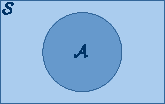
\includegraphics[width=0.7\linewidth]{./Graphics/VennDiag_1.pdf}
    \caption{Venn diagram representation of an event $\mathcal{A}$
    residing on sample space $\mathcal{S}$}\label{fig:1}
    \end{Figure}

    \begin{definition}[Naive definition of probability]
        Assuming that
        \begin{enumerate}
            \item all outcomes are equally likely, and
            \item sample space $\mc{S}$ is finite,
        \end{enumerate}
        the probability that $\mc{A}$ occurs is given by
        \begin{align}
            P(\mc{A}) &= \dfrac{\text{\# favorable outcomes}}{\text{\# possible
            outcomes}}
        \end{align}
    \end{definition}

    Assumption 2 is needed otherwise all the probabilities are zero. Assumption
    1 is a rather strong assumtion which is true in many cases but not all.
    Mostly in problems which involves some kind of {\em symmetry}, assumption 1
    holds nice, e.g., a fair coin, a fair dice.

    \subsection{Extreme of failure of Naive definition}
    \begin{itemize}
        \item The possibility of life on Neptune is $\frac{1}{2}$.
        \item The possibility of intelligent life on Neptune is also
            $\frac{1}{2}$. Should it not be strictly less than all life?
            Absurdity!
    \end{itemize}
    Always need some justification to apply naive definition. Especially,
    adherance to the above two assumptions.

    \section{Basic principles of counting}
    To be able to use the naive definition of probability, we should be able to
    count. Let us introduce {\em multiplication rule} to do this.

    \begin{proposition}[Multiplication Rule]
        If there are $r$ number of experiments and each experiment has $n_i$
        number of possible outcomes, then the overall sample space has size
        \begin{align}
            |\mc{S}| &= \prod\limits_{i=1}^r n_i
        \end{align}
    \end{proposition}

    \begin{Figure}
        \centering
        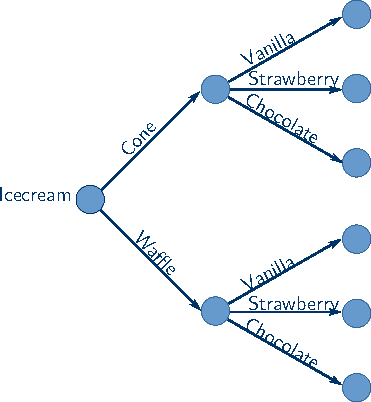
\includegraphics[width =
        0.9\linewidth]{./Graphics/MultiplicationRule.pdf}
        \caption{The icecream coutning tree explanning multiplication rule}
        \label{fig2}
    \end{Figure}

    \begin{example}
        The probability of a full house (e.g., three 7s and two Jacks) in a five
        card poker hand (without replacement, and without other players) is
        \begin{align}
            P(\text{full house}) &= \dfrac{13\times \dbinom{4}{3}\times 12\times
            \dbinom{4}{2}}{\dbinom{52}{5}}
        \end{align}
    \end{example}

    \begin{definition}[Binomial Coefficient]
        The binomial coefficient is given by
        \begin{align}
            \dbinom{n}{k} &= \left\{
            \begin{array}{lc}
                \dfrac{n!}{(n-k)!\ k!}, & n\ge k\\\\
                0, & \text{otherwise.}
            \end{array}
            \right.
        \end{align}
    \end{definition}

    \begin{theorem}[Sampling Table]
        \begin{table}
        \centering
        \caption{Please write your table caption here}
        \label{tab:1}       % Give a unique label
        %
        % For LaTeX tables use
        %
        \begin{tabular}{lll}
        \hline\noalign{\smallskip}
        first & second & third  \\
        \noalign{\smallskip}\hline\noalign{\smallskip}
        number & number & number \\
        number & number & number \\
        \noalign{\smallskip}\hline
        \end{tabular}
        \end{table}
        %

    \end{theorem}


%
\section{Section Heading}
\label{sec:1}
% Always give a unique label
% and use \ref{<label>} for cross-references
% and \cite{<label>} for bibliographic references
% use \sectionmark{}
% to alter or adjust the section heading in the running head
Your text goes here. Use the \LaTeX\ automatism for your citations
\cite{monograph}.

\subsection{Subsection Heading}
\label{sec:2}
Your text goes here.

\begin{equation}
\vec{a}\times\vec{b}=\vec{c}
\end{equation}

\subsubsection{Subsubsection Heading}
Your text goes here. Use the \LaTeX\ automatism for cross-references as
well as for your citations, see Sect.~\ref{sec:1}.

\paragraph{Paragraph Heading} %
Your text goes here.

\subparagraph{Subparagraph Heading.} Your text goes here.%
%
\index{paragraph}
% Use the \index{} command to code your index words
%
% For tables use
%
\begin{table}
\centering
\caption{Please write your table caption here}
\label{tab:1}       % Give a unique label
%
% For LaTeX tables use
%
\begin{tabular}{lll}
\hline\noalign{\smallskip}
first & second & third  \\
\noalign{\smallskip}\hline\noalign{\smallskip}
number & number & number \\
number & number & number \\
\noalign{\smallskip}\hline
\end{tabular}
\end{table}
%
%
% For figures use
%
% For built-in environments use
%
\begin{theorem}
Theorem text goes here.
\end{theorem}
%
% or
%
\begin{lemma}
Lemma text goes here.
\end{lemma}
%
%
% Problems or Exercises should be sorted chapterwise
\section*{Problems}
\addcontentsline{toc}{section}{Problems}
%
% Use the following environment.
% Don't forget to label each problem;
% the label is needed for the solutions' environment
\begin{prob}
\label{prob1}
The problem\footnote{Footnote} is described here. The
problem is described here. The problem is described here.
\end{prob}

\begin{prob}
\label{prob2}
\textbf{Problem Heading}\\
(a) The first part of the problem is described here.\\
(b) The second part of the problem is described here.
\end{prob}

(b) The second part of the problem is described here.
(b) The second part of the problem is described here.
(b) The second part of the problem is described here.
(b) The second part of the problem is described here.
(b) The second part of the problem is described here.
(b) The second part of the problem is described here.
(b) The second part of the problem is described here.
(b) The second part of the problem is described here.
(b) The second part of the problem is described here.
(b) The second part of the problem is described here.
(b) The second part of the problem is described here.
(b) The second part of the problem is described here.
(b) The second part of the problem is described here.
(b) The second part of the problem is described here.
(b) The second part of the problem is described here.
(b) The second part of the problem is described here.
(b) The second part of the problem is described here.
(b) The second part of the problem is described here.
(b) The second part of the problem is described here.
(b) The second part of the problem is described here.
(b) The second part of the problem is described here.
(b) The second part of the problem is described here.
(b) The second part of the problem is described here.
(b) The second part of the problem is described here.
(b) The second part of the problem is described here.
(b) The second part of the problem is described here.
(b) The second part of the problem is described here.
(b) The second part of the problem is described here.
(b) The second part of the problem is described here.
(b) The second part of the problem is described here.
(b) The second part of the problem is described here.
(b) The second part of the problem is described here.
(b) The second part of the problem is described here.
(b) The second part of the problem is described here.
(b) The second part of the problem is described here.
(b) The second part of the problem is described here.
(b) The second part of the problem is described here.
(b) The second part of the problem is described here.
(b) The second part of the problem is described here.
(b) The second part of the problem is described here.
(b) The second part of the problem is described here.
(b) The second part of the problem is described here.
(b) The second part of the problem is described here.
(b) The second part of the problem is described here.
(b) The second part of the problem is described here.
(b) The second part of the problem is described here.
(b) The second part of the problem is described here.
(b) The second part of the problem is described here.
(b) The second part of the problem is described here.
(b) The second part of the problem is described here.
(b) The second part of the problem is described here.
(b) The second part of the problem is described here.
(b) The second part of the problem is described here.
(b) The second part of the problem is described here.
(b) The second part of the problem is described here.
(b) The second part of the problem is described here.
(b) The second part of the problem is described here.
(b) The second part of the problem is described here.
(b) The second part of the problem is described here.
(b) The second part of the problem is described here.
(b) The second part of the problem is described here.
(b) The second part of the problem is described here.
(b) The second part of the problem is described here.
(b) The second part of the problem is described here.
(b) The second part of the problem is described here.
(b) The second part of the problem is described here.
(b) The second part of the problem is described here.
(b) The second part of the problem is described here.
(b) The second part of the problem is described here.
(b) The second part of the problem is described here.
(b) The second part of the problem is described here.
(b) The second part of the problem is described here.
(b) The second part of the problem is described here.
(b) The second part of the problem is described here.
(b) The second part of the problem is described here.
(b) The second part of the problem is described here.
(b) The second part of the problem is described here.
(b) The second part of the problem is described here.
(b) The second part of the problem is described here.
(b) The second part of the problem is described here.
(b) The second part of the problem is described here.
(b) The second part of the problem is described here.
(b) The second part of the problem is described here.
(b) The second part of the problem is described here.
(b) The second part of the problem is described here.
(b) The second part of the problem is described here.
(b) The second part of the problem is described here.
(b) The second part of the problem is described here.
(b) The second part of the problem is described here.
(b) The second part of the problem is described here.
(b) The second part of the problem is described here.
(b) The second part of the problem is described here.
(b) The second part of the problem is described here.
(b) The second part of the problem is described here.
(b) The second part of the problem is described here.
(b) The second part of the problem is described here.
(b) The second part of the problem is described here.
(b) The second part of the problem is described here.
(b) The second part of the problem is described here.
(b) The second part of the problem is described here.
(b) The second part of the problem is described here.
(b) The second part of the problem is described here.
(b) The second part of the problem is described here.
(b) The second part of the problem is described here.
(b) The second part of the problem is described here.
(b) The second part of the problem is described here.
(b) The second part of the problem is described here.
(b) The second part of the problem is described here.
(b) The second part of the problem is described here.
(b) The second part of the problem is described here.
(b) The second part of the problem is described here.
(b) The second part of the problem is described here.
(b) The second part of the problem is described here.
(b) The second part of the problem is described here.
(b) The second part of the problem is described here.
(b) The second part of the problem is described here.
(b) The second part of the problem is described here.
(b) The second part of the problem is described here.

\end{multicols}
%
